\documentclass[journal]{IEEEtran}
\usepackage{graphicx}
\usepackage{hyperref}
\hyphenation{op-tical net-works semi-conduc-tor}

\usepackage{listings}
\usepackage{color}

\definecolor{dkgreen}{rgb}{0,0.6,0}
\definecolor{gray}{rgb}{0.5,0.5,0.5}
\definecolor{mauve}{rgb}{0.58,0,0.82}

\lstset{frame=tb,
  language=Matlab,
  aboveskip=3mm,
  belowskip=3mm,
  showstringspaces=false,
  columns=flexible,
  basicstyle={\small\ttfamily},
  numbers=none,
  numberstyle=\tiny\color{gray},
  keywordstyle=\color{blue},
  commentstyle=\color{dkgreen},
  stringstyle=\color{mauve},
  breaklines=true,
  breakatwhitespace=true,
  tabsize=3
}

\begin{document}

\title{The N-Robot Formation and Path Tracking Procedure}
\author{\textit{Ben~Cannon}, \textit{Eric~Wallace}, \textit{Omar~Abdelkader}}

\maketitle

\begin{abstract}
    The main purpose of this technical report is to describe an optimal solution to the n-robot formation and path tracking procedure problem. In this problem, \textit{n} randomly placed identical autonomous robots are tasked with locating one another, lining up in formation, and moving along a path following the "leader", or first robot.
\end{abstract}

\begin{IEEEkeywords}
    Dubins car, pure pursuit, differential drive, autonomous navigation, target pose.
\end{IEEEkeywords}

\section{Introduction}
    Consider a room filled with N differential drive robots [2]. We will be required to design a communication system and control algorithm that causes the robots to form a line at an arbitrary point in the room, and then follow an arbitrary path.
    
    The following constraints are placed on our robot formation system:
    
    \begin{enumerate}
        \item The robots are not assigned a trivial ordering.
            \begin{itemize}
                \item There is no physical labeling of the cars.
                \item The robots' ordering cannot be hard-coded into their firmware.
                \item No determination of order can be made by the serial number or any other physical attribute.
            \end{itemize}
        \item No robot is trivially assigned as leader.
            \begin{itemize}
                \item Each robot has equal rights or priority to be the leader.
            \end{itemize}
        \item All the robots communicate with each other via an exclusive network where they can share information (i.e. position and heading) with one another.
    \end{enumerate}
    
    In brief, this problem is comparable to parents asking their identical children with the same name to form a line and follow a trajectory.

\subsection{Dubins Car}
    We will model our robots after a Dubins car. These cars have two wheels on either side of the car body, with a simple motor powering each. In our system, we will be ignoring any collisions amongst cars. We will also consider a room with no obstacles inside.

    \centerline{
\includegraphics[width=0.90in,height=0.90in,clip]{dubin_car}}
    \centerline{\textit{Fig:1 Dubins Car}}
    
    By driving the motors at the same angular velocity, we can propel the car forward. By driving the motors at equal but opposite angular velocities, we can rotate the car in place. Combining these two forms of motion provides the robot with a third form of motion, traveling in a curved line or path.

\subsection{State Space}
    The only factor that differentiates one robot from another is the robot's state. Each robot is defined by its position $\left(x,y\right)$ and its heading angle $\left(\Theta\right)$. Taken together, we call the state vector $\left(x\left(t\right),y\left(t\right),\Theta\left(t\right)\right)$ the robot's "pose" at time t.
    
    If we define $U_{L}$ and $U_{R}$ to be the wheel speeds of the right and left wheels, respectively, then the robot's equations of motion are governed by:
    
    \begin{center}
        $\dot{x} = \frac{r}{2}\left(U_{L}+U_{R}\right)\cos(\Theta)$ \\
        $\dot{y} = \frac{r}{2}\left(U_{L}+U_{R}\right)\sin(\Theta)$ \\
        $\dot{\Theta} = \frac{r}{L}\left(U_{L}-U_{R}\right)$
    \end{center}
        
    Here, \textit{r} is the radius of the wheels and \textit{L} is the distance between the wheels. The wheel speeds $U_{L}$ and $U_{R}$ are the "controls", or inputs to the system, that allow us to maneuver the robot [3].
    
    It is important to note that the differential robot is \textit{completely controllable}, meaning that any final pose can be reached from any initial pose. Upon further inspection, this is immediately clear. Although it would not always be the most efficient means of travel, a robot can travel between any two configurations by 1) rotating itself to the goal position; 2) translating to the goal position; 3) and rotating itself to the desired final orientation.

\section{Navigation Algorithm}
    \centerline{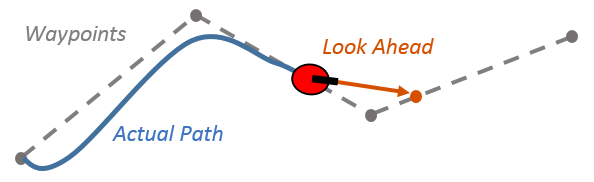
\includegraphics[width=2.5in,height=1in,clip]{Lookahead}}
    \centerline{\textit{Fig:2 Lookahead Method [4]}}
    
    The most obvious means of navigation between two points would be to implement the "turn and shoot" method. In this procedure, the robot orients itself so that its heading is towards the goal point and drives forwards until it reaches that coordinate. This process can be repeated as many times as necessary in order to follow a set of waypoints or path. While easy to implement in a computational software package like MATLAB, this path tracking technique requires frequent stopping and starting. As the car's heading begins to divert from its goal, the car will stop proceeding forward and begin a rotation. This leads to an undesirable and unrealistic "inchworm" type movement, which occurs especially often when the robot must turn at a sharp angle.
    
    The pure pursuit algorithm (using an adaptive look-ahead distance), which we choose to utilize in our simulations, solves many of the problems presented by the "turn and shoot" technique. Although there are several procedures that may be better suited for the problem being presented, pure pursuit is one of the more efficient algorithms for its level of implementation complexity.
    
    In this algorithm the robot looks ahead along the path it is following and identifies a point one look-ahead distance, \textit{D}, away from its current position. This look-ahead distance parameter is adapted based on the robots current distance from the path it is tracking [1]. For example, when the robot is right on the path its look-ahead distance will be small for accurate path tracking, but when it is far off the current planned trajectory it will increase to allow the robot to regain the path.  This offers far better stability than using a fixed look-ahead distance [1]. After identifying a look-ahead distance, the robot calculates the curvature of an arc that it must follow in order to reach the goal position [1].
    
    The robot uses this look-ahead distance and curvature to determine its controls (the setting of the angular velocity of the left and right motors). The following code snippet illustrates the methodology for determining the left and right arc drive control laws; where \textit{rNear} is the interior wheel radius of the turn and \textit{rFar} is the exterior wheel radius of the turn and are determined by subtracting $\frac{L}{2}$ (for \textit{rNear}) and adding $\frac{L}{2}$ (for \textit{rFar}) from the radius of the curve calculated using the pure pursuit algorithm.
        
    \begin{lstlisting}
        % turn left
        if(strcmp(direction, 'left'))
            UR = veloctiy;
            UL = (rNear/rFar)*UR;
        % turn right
        elseif(strcmp(direction, 'right'))
            UL = velocity;
            UR = (rNear/rFar)*UL;
        end
    \end{lstlisting}
        
    One of the issues with pure pursuit is when the robot is facing the opposite heading of where it needs to travel to. In this case, the robot will attempt to follow a extremely long, sweeping pattern to circle around to its target heading. Moreover, pure pursuit is intended to be constantly looking ahead to a goal point, and thus causes inconsistent behavior when approaching the end of a path. In order to remedy this, we formed a combination of the "turn and shoot" and adaptive look ahead pure pursuit algorithm.  
    
    We first initiate "orient mode", where the robot simply rotates to face the correct heading towards its first goal point. The robot then continually operates the pure pursuit algorithm to track and follow the path until it approaches the end of the path. It finally enters "finish mode", where the robot uses "turn and shoot" to reach its final point with great accuracy. 

\section{Formation Algorithm}
    Prior to following a path, the robots must align themselves in formation, starting at the first waypoint in the path. The ordering of the robots is determined by calculating their respective distances from said starting point. For example, the robot closest to the start of the path will be assigned the first position, or "leader", of the formation. The robot second closest to the initial point is assigned the second position, and so on until the last robot is assigned its position in the formation.\\
    
    \centerline{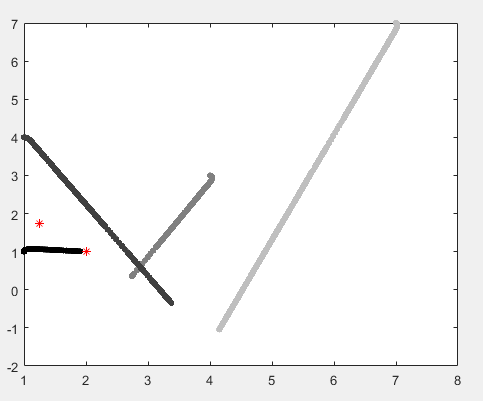
\includegraphics[width=3in,height=3in,clip]{formation}}
    \centerline{\textit{Fig:3 Formation}}
    
    Using this procedure, the robots will form a line at the start of the path, positioning themselves on 1 meter intervals along the tangential vector connecting the first and second waypoints. The figure above depicts a MATLAB simulation of the formation algorithm in effect. It shows four robots lining up along the vector connecting the first waypoint, $\left(2.00,1.00\right)$, and  second waypoint, $\left(1.25,1.75\right)$ of the path. Once all the robots are in proper formation, the "leader" can begin efficiently tracking the target path while the remaining robots will track the robot preceding it in the formation.

\section{Path Tracking and Robot Following}
    Once each robot is in position, a signal flag will be raised to indicate that all the robots have successfully assembled in formation. Upon receiving the signal, the "leader" will begin to follow the pure pursuit algorithm and track the path using the control system described in the \textit{Navigation Algorithm} section.
    
    Rather than tracking the path, the remaining robots, who will be referred to as "followers", will track the position of the robot immediately preceding it. The path tracking algorithm used by the "follower" robots is simply a condensed version of the "leader" algorithm. In the "follower" edition, the same algorithm is run using a two-waypoint path, $\left[current~position,~preceding~robot~position\right]$, and goal point one look-ahead distance on the path. In this implementation, each "follower" robot will be tracking the robot directly in front of it.

\section{The Simulation}
    We used MATLAB to create a simulation of five different scenarios. The code used to generate this simulation is available on GitHub at the following link \url{https://github.com/omikader/robot-formation}. The five simulations are as follows:
    
    \begin{enumerate}
        \item An open loop control system. In this scenario, the robot won't use the pure pursuit algorithm, it will simply demonstrate different driving mechanics. The robot drives straight, makes a turn, and then continues straight on a different trajectory.
        \item Navigation to a target pose. In this scenario, the robot must maneuver to a target point and orient to a target heading. We use the adaptive look ahead pure pursuit algorithm to navigate the robot to the point.  
        \item An arbitrary target path. In this scenario, the robot will following the described navigation algorithm to reach the start of the path, track the path's trajectory, and position itself on the final point.  
        \item Two robots that follow an arbitrary target path. In this scenario, the robots will determine their line position and navigate to their respective positions in the line. The "leader" robot will then track the path trajectory, while the "following" robot will track the position of the leader.
        \item N robots follow an arbitrary target path. The robots will calculate their order, create the line formation, and assign a leader and followers. The leader will then track the path, while each follower is tracking the robot directly in front of it.\\
    \end{enumerate}
    
    \centerline{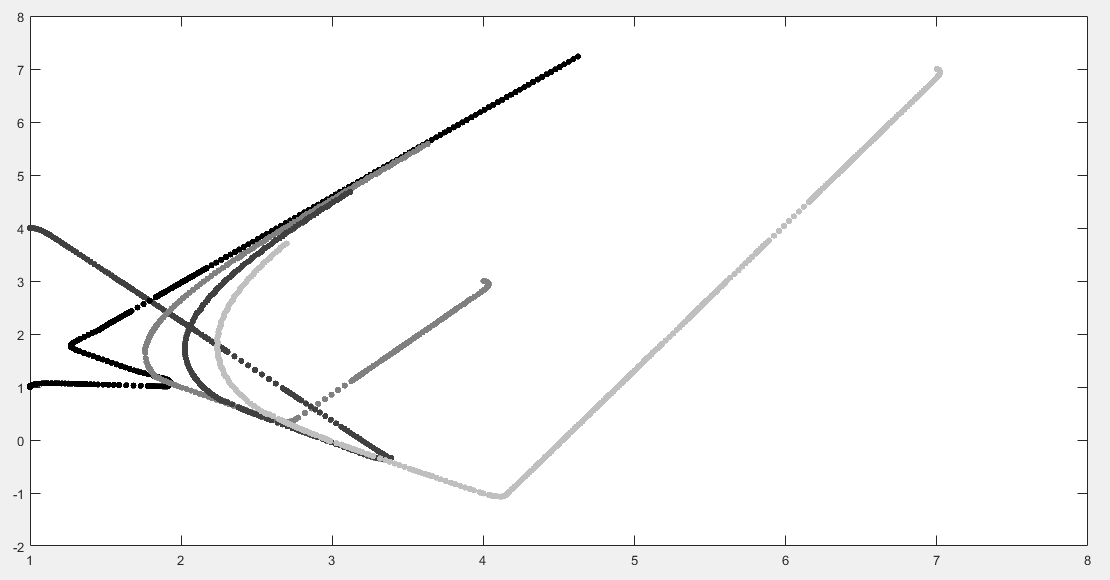
\includegraphics[width=3in,height=3in,clip]{simulation}}
    \centerline{\textit{Fig:4 Simulation 5}}
    
    The figure above shows a screen shot of simulation number five of our control method run for four robots, set at different starting points. The robots trajectories are mapped on an $\left(x,y\right)$ grid and the pure pursuit with adaptive look-ahead algorithm is used to track the desired path.

\section{Conclusions and Suggestions for Further Research}
    In this procedure, we provide a method for a collection of N robots to form a single file line formation and track a path trajectory as a group. We have presented a method to track path's using a combination of the "turn and shoot" and the adaptive look ahead pure pursuit algorithms. Furthermore, we have described a method for the robots to determine their relative position in line, and calculate their respective initial starting position. Using a combination of intercommunication and control systems, we were able to create a complex simulation of N-robots organizing themselves and tracking a leader's trajectory.
    
    In this paper, we assume that the robots are free to move over any area in the $\left(x,y\right)$ plane by neglecting the event of robot collisions or the presence of obstacles. As a result, this implementation does not handle situations in which a robot can get separated from the pack. We also disregard acceleration in the robot's wheels. Creating an improved simulation that takes advantage of these factors will provide more realistic applications for the described problems. Other tracking and following algorithms that use a PID-based controller could be implemented to more accurately track the leading robot.

\section*{Acknowledgment}
    We would like to thank Dr. Blankenship for the guidance throughout the semester in our Signals and Systems Course.

\section*{References}
    [1] Giesbrecht, J., D. Mackay, J. Collier, and S. Verret. "Path Tracking for Unmanned Ground Vehicle Navigation." Defence Research and Development Canada, December 2005. 
    
    [2] Lavelle, Steven M. "A Differential Drive Robot." Algorithms. Accessed December 12, 2016. http://planning.cs.uiuc.edu/node659.html.
    
    [3] Lundgren, Martin. "Path Tracking for a Miniature Robot." Master's thesis, Umea University, 2003. Accessed December 12, 2016. http://www8.cs.umu.se/kurser/TDBD17/VT06/utdelat/Assignment Papers/Path Tracking for a Miniature Robot.pdf.
    
    [4] Mathworks. "Pure Pursuit Controller." Pure Pursuit Controller - MATLAB \& Simulink. Accessed December 12, 2016. https://www.mathworks.com/help/robotics/ug/pure-pursuit-controller.html.
        
\end{document}